\section{What is Virtual Reality?}
The \textbf{definition of virtual reality} comes, naturally, from the definitions for both "virtual" and "reality". The definition of "virtua"’ is near and reality is what we experience as human beings. So the term ""virtual reality"" basically means "near-reality". This could, of course, mean anything but it usually refers to a specific type of reality emulation.

We know the world through our senses and perception systems. In school we all learned that we have five senses: taste, touch, smell, sight and hearing. These are however only our most obvious sense organs. The truth is that humans have many more senses than this, such as a sense of balance for example. These other sensory inputs, plus some special processing of sensory information by our brains ensures that we have a rich flow of information from the environment to our minds.

Everything that we know about our reality comes by way of our senses. In other words, our entire experience of reality is simply a combination of sensory information and our brains sense-making mechanisms for that information. It stands to reason then, that if you can present your senses with made-up information, your perception of reality would also change in response to it. You would be presented with a version of reality that isn’t really there, but from your perspective it would be perceived as real. Something we would refer to as a virtual reality.

So, in summary, virtual reality entails presenting our senses with a computer generated virtual environment that we can explore in some fashion.

\begin{figure}[!h]
	\begin{center}
		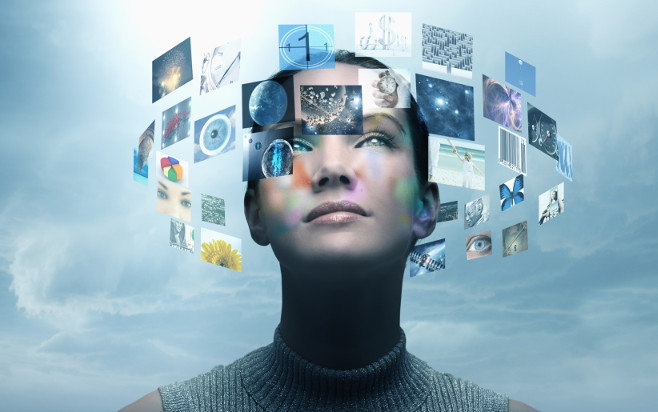
\includegraphics[width=1\linewidth]{images/vr_women}
		\caption{Women designed with VR}
	\end{center}
\end{figure}


\section{Techincal term behind VR}

Answering "what is virtual reality" in technical terms is straight-forward. Virtual reality is the term used to describe\textbf{ a three-dimensional, computer generated environment} which can be explored and interacted with by a person. That person becomes part of this virtual world or is immersed within this environment and whilst there, is able to manipulate objects or perform a series of actions.

\section{How is virtual reality achieved?}

Although we talk about a few historical early forms of virtual reality elsewhere on the site, today virtual reality is usually implemented using computer technology. There are a range of systems that are used for this purpose, such as headsets, omni-directional treadmills and special gloves. These are used to actually stimulate our senses together in order to create the illusion of reality.

This is more difficult than it sounds, since our senses and brains are evolved to provide us with a finely synchronized and mediated experience. If anything is even a little off we can usually tell. This is where you’ll hear terms such asimmersiveness  and realism enter the conversation. These issues that divide convincing or enjoyable virtual reality experiences from jarring or unpleasant ones are partly technical and partly conceptual. Virtual reality technology needs to take our physiology into account. For example, the human visual field does not look like a video frame. We have (more or less) 180 degrees of vision and although you are not always consciously aware of your peripheral vision, if it were gone you’d notice. Similarly when what your eyes and the vestibular system in your ears tell you are in conflict it can cause motion sickness. Which is what happens to some people on boats or when they read while in a car.

If an implementation of virtual reality manages to get the combination of hardware, software and sensory synchronicity just right it achieves something known as a sense of presence. Where the subject really feels like they are present in that environment.

\begin{figure}[!h]
	\begin{center}
		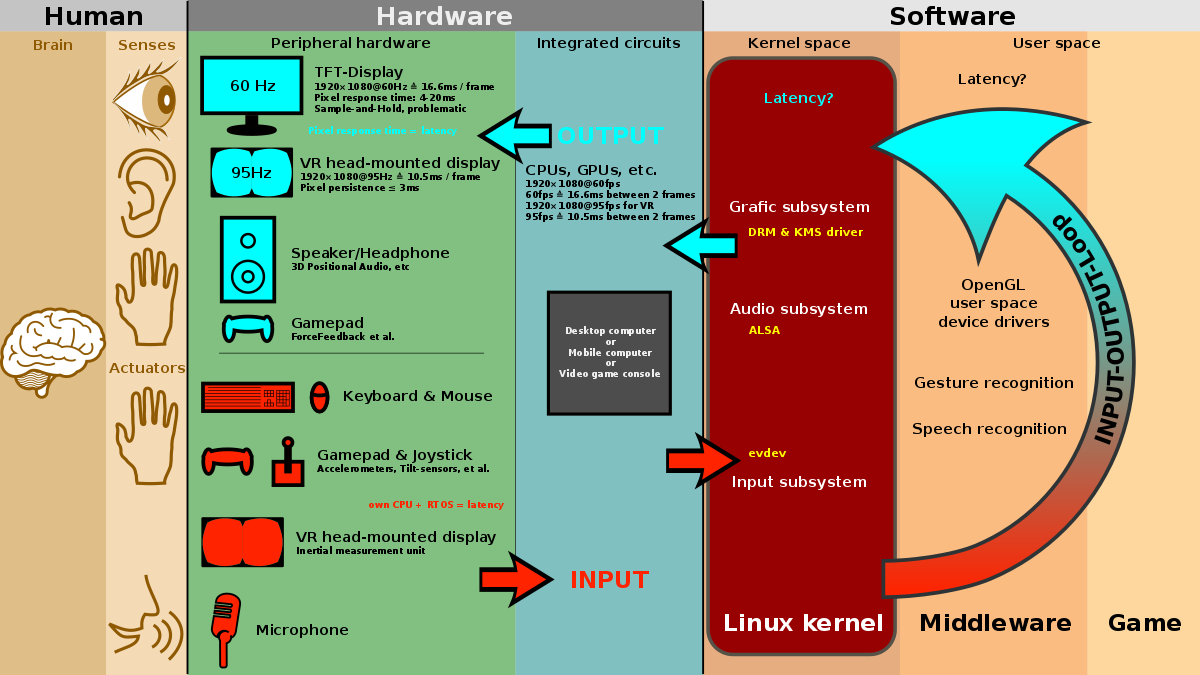
\includegraphics[width=0.7\linewidth]{images/vr_desc}
		\caption{Description of the functionality of VR}
	\end{center}
\end{figure}

\newpage
\section{Why have virtual reality?}

This may seems like a lot of effort, and it is! What makes the development of virtual reality worthwhile? The potential entertainment value is clear. Immersive films and video games are good examples. The entertainment industry is after all a multi-billion dollar one and consumers are always keen on novelty. Virtual reality has many other, more serious, applications as well.

There are a wide variety of applications for virtual reality which include:

\begin{itemize}
	\item Architecture
	\item Sport
	\item Medicine
	\item The Arts
	\item Enterainment
\end{itemize}

Virtual reality can lead to new and exciting discoveries in these areas which impact upon our day to day lives.

Wherever it is too dangerous, expensive or impractical to do something in reality, virtual reality is the answer. From trainee fighter pilots to medical applications trainee surgeons, virtual reality allows us to take virtual risks in order to gain real world experience. As the cost of virtual reality goes down and it becomes more mainstream you can expect more serious uses, such as education or productivity applications, to come to the fore. Virtual reality and its cousin augmented reality could substantively change the way we interface with our digital technologies. Continuing the trend of humanising our technology.


\section{How Virtual Reality is being used today}

Unsurprisingly, the video games industry is one of the largest proponents of Virtual Reality. Support for the Oculus Rift headsets has already been jerry-rigged into games like Skyrim and Grand Theft Auto , but newer games like Elite: Dangerous come with headset support built right in. Many tried-and-true user interface metaphors in gaming have to be adjusted for VR (after all, who wants to have to pick items out of a menu that takes up your entire field of vision?), but the industry has been quick to adapt as the hardware for true Virtual Reality gaming has become more widely available.

\newpage
	\subsection{Virtual Reality and data visualization}

	Scientific and engineering data visualization has benefited for years from Virtual Reality, although recent innovation in display technology has generated interest in everything from molecular visualization to architecture to weather models.

	\subsection{VR for aviation, medicine and the military}
	
	In aviation, medicine, and the military, Virtual Reality training is an  attractive alternative to live training with expensive equipment, dangerous situations, or sensitive technology. Commercial pilots can use realistic cockpits with VR technology in holistic training programs that incorporate virtual flight and live instruction. Surgeons can train with virtual tools and patients, and transfer their virtual skills into the operating room, and studies have already begun to show that such training leads to faster doctors who make fewer mistakes. Police and soldiers are able to conduct virtual raids that avoid putting lives at risk.
	
	\subsection{Virtual Reality and the treatment of mental illness}
	
	Speaking of medicine, the treatment of mental illness, including post-traumatic stress disorder, stands to benefit from the application of Virtual Reality technology to ongoing therapy programs. Whether it’s allowing veterans to confront challenges in a controlled environment, or overcoming phobias in combination with behavioral therapy, VR has a potential beyond gaming, industrial and marketing applications to help people heal from, reconcile and understand real world experiences.

\section{Features of virtual reality systems}

There are many different types of virtual reality systems but they \textbf{all share the same characteristics} such as the ability to allow the person to \textbf{view three-dimensional images}. These images appear life-sized to the person.

Plus they change as the person moves around their environment which corresponds with the change in their field of vision. The aim is for a seamless join between the person’s head and eye movements and the appropriate response, e.g. change in perception. This ensures that the virtual environment is both realistic and enjoyable.

A virtual environment \textbf{should provide the appropriate responses} – in real time- as the person explores their surroundings. The problems arise when there is a delay between the person’s actions and system response or latency which then disrupts their experience. The person becomes aware that they are in an artificial environment and adjusts their behaviour accordingly which results in a stilted, mechanical form of interaction.

The aim is for a natural, free-flowing form of interaction which will result in a memorable experience.

\newpage
\section{Top Virtual Reality technology trends for 2016}

	\subsection{First Taste for private Persons}
	
	Consumers won’t have to pay for their initial AR and VR experiences. Sponsored experiences are driving initial desire and market adoption before VR headsets become a part of the average person’s tech arsenal. From the New York Times and ABC News to “Star Wars” and the Lowe’s Holoroom, we will continue to see big media, entertainment and retail brands test the limits of VR and AR tech with sponsored experiences that reach millions of consumers and expose unlikely audiences to Virtual and Augmented Reality. And it will be free for now.
	
	\subsection{Hololens for gaming}
	
	Over the past few years, hardware has dominated the conversation around Virtual Reality and Augmented Reality. There have been big ideas and slick gaming demos, one notable failure (Google Glass) and a lot of crazy weird entries to the category. There have been recent daring investments in mysterious companies like Magic Leap, and the gobbling up of intellectual property by behemoths like Google, Facebook and Apple. 2016 promises major new releases, including the Facebook-owned Oculus Rift (now available though very hard to find), the HTC Vive, Microsoft HoloLens, and branded headsets to pair with Sony PlayStation 4 and Microsoft Xbox One. Many of the new units are pricey (Oculus is \$599, the Vive is \$799, and the HoloLens will set you back a hefty \$3,000), but there are other hardware options now available at a more accessible price point. Samsung GearVR runs a remarkably affordable \$99.99, and recent promotions saw GearVR being given away with the purchase of a Galaxy S7 smartphone. Google Cardboard can be yours for as little as \$1.50 (or even free in some cases), the low price helping Google move more than five million Cardboard sets into the hands of consumers.

\section{Conclusion}
Virtual reality is the creation of a virtual environment presented to our senses in such a way that we experience it as if we were really there. It uses a host of technologies to achieve this goal and is a technically complex feat that has to account for our perception and cognition. It has both entertainment and serious uses. The technology is becoming cheaper and more widespread. We can expect to see many more innovative uses for the technology in the future and perhaps a fundamental way in which we communicate and work thanks to the possibilities of virtual reality.
